\chapter{Introduction}

Everyday, humans generate a huge set of information while interacting with the internet, especially since the era of the
Internet of Things (IoT). This data is often going to be discarded, sometimes it might be logged, but even then in most
cases there is no further usage. Tasks like storing data and logging are considered tedious and receive little attention
in addition to the actual programming work.

However, this is precisely the kind of data which is relevant for data science topics like the optimisation of an existing
business process with a cognitive model or the exploration of lucrative new business fields to invest in.

\section{Project Overview}

Mobi24 is an assistance and emergency call centre founded by the Swiss Mobiliar in 1997. It's the initial touch point for
clients and potential future clients. Most of the in-going requests are about insurance related subjects. The purpose of
this bachelor thesis is the creation of a natural language model for named-entity recognition in the insurance context
based on client data from Mobi24. There exist several pretrained models which are free to use, but just a few of them are
capable of dealing with the German language and none of them are trained with insurance data. In the future, the final model
should help the data scientists at Swiss Mobiliar for their own specific \acrshort{nlp}\footnote{Natural Language Processing deals
with the understanding of human languages} tasks. The most interesting named entities for Swiss Mobiliar are the people's names
and their addresses.

\subsection{Benefits}

A reasonable \acrshort{ner} model will give the Swiss Mobiliar several benefits in understanding natural language and thereby
offering an even better service to its customers. The future model should be available as a python library in the Swiss Mobiliar
repository. If this model fits any data scientist's needs, he should take advantage of it.

Due to limited time resources the final model should only recognise names and addresses. It's possible to extend the list of named
entities with new values like phone numbers or insurance polices.

\subsubsection{Parameter Space and Complexity}

The main advantage of such a model is to create suitable data to reduce the parameter space of any other language model. With a
reduced parameter space, the size of the model itself and it's training duration gets minimised. Especially if you want to develop
micro services, a lightweight and therefore fast model is required to satisfy customers needs.

Table \ref{tbl:param-space} shows, that the reduced parameter space consists of much less tokens than the original space. In this
case it uses only $\frac{4}{7}$ of the tokens to express nearly the same amount of information. For a model, which wants to learn
user's intents and doesn't need the plain facts, this would be a real advantage. Of course there are plenty of other examples.

\begin{table}[h!]
    \centering
    \begin{tabular}{|l|c|c|c|c|c|c|c|}
        \hline
        \textbf{Default} & Sherlock & Holmes & lives & at & 221b & Baker & Street. \\
        \hline
        \textbf{Reduced} & PER & lives & at & LOC & & & \\
        \hline
    \end{tabular}
    \caption{Comparison of two parameter spaces}
    \label{tbl:param-space}
\end{table}

\subsubsection{Anonymisation}

Additionally, the model will be used to create anonymised data. The cleaned data could be used for demonstration purposes. Even
training in a cloud-based infrastructure would be significantly easier because of zero restrictions from data policies. All data
processed by the \acrshort{ner} model can be freely distributed across Swiss Mobiliar.

Instead of removing personal information there is also the opportunity to replace named entities with fictional values. The data
would look correctly but isn't mirroring the reality and thus can be shared again. Although this approach may confuse users which
aren't aware of the fact that the entities are fictional it's worth mentioning.

Though it's important to keep in mind that real anonymisation isn't possible. After data is being de-identified\footnote{The process
of anonymising personal data} it can be used and shared without the restrictions of data protection laws. Sharing research data
across institutions boosts the development of scientific inventions. The problem is that the data only seems to be anonymised. In
fact, there is a high chance to recognise individuals if the data is being populated with additional data sources \cite{rocher19}.
Imagine a de-identified insurance case about a car accident. There's the possibility to simply search news sites for car accidents at
the concrete date to get personal information about the vehicle type or even the owner.

\subsubsection{Form Completion}

In information extraction, such a model can be useful to localise user data and complete a form with the extracted parts. If
you combine the model with an intent classifier\footnote{A model to predict user intents, widely used in smart assistants},
a very powerful combination arises \cite{jain18}. You could create pre-filled insurance offers from client requests. This would
speed up the process and may result in more sales. Swiss Mobiliar is actually doing research on chat bot like claim classifiers to
automatically recognise different type of claims.

\subsection{Objectives}

For a successful completion of the bachelor thesis several deliverables need to be offered to the stakeholders. Additionally
to this document there should exist a functioning language model with an anonymized training data set. This training set
should have an appropriate size for training the model and comparing the different outcomes. The source code should be
written under consideration of the commonly known software engineering and design patterns. The model is developed
iteratively with one or more baseline models at beginning. The goal is to optimise the model with every new approach to
get the highest possible recognition rate.

From an administrative point of view there needs to be a presentation in the middle of January. Furthermore an abstract, used
for the BFH publication of all bachelor theses, a poster of size A3, and a short movie clip are expected.

\subsection{Stakeholders}

There are several stakeholders interested in the outcome of this project. There would be, for example, the Swiss Mobiliar and
especially its data scientists, who want to reuse the trained NLP model for their own projects. On the other hand, there is
the Bern University of Applied Sciences which is demanding a satisfactory thesis for awarding me with the bachelor's degree
in computer science. Last but not least, I act as a stakeholder as well and I want to dig deeper in the field of data science and
learn as much as possible. It will be challenging to satisfy all these different stakeholders to an adequate level.

\subsection{Submission Deadlines}

This bachelor thesis is carried out in compliance with various deadlines. Table \ref{tbl:deadlines} gives an insight about the most
relevant milestones and when they should be delivered to the stakeholders.

\begin{table}[ht!]
    \centering
    \begin{tabular}{|l|l|}
        \hline
        \textbf{Date} & \textbf{Submissions and Milestones} \\ [0.5ex]
        \hline
        16.09.2019 & Begin of semester, project kick off \\
        03.01.2020 & Submission of poster (A3) \\
        16.01.2020 & Submission of report, movie clip \\
        17.01.2020 & Presentation at BFH Techday \\
        17.01.2020 & Poster exhibition \\
        07.02.2020 & Grading conference \\
        06.03.2020 & Graduation party \\ [1ex]
        \hline
    \end{tabular}
    \caption{Most important (submission) dates}
    \label{tbl:deadlines}
\end{table}

\section{Data Sources}

The future NLP model relies on two distinctive data sources. In detail, there is a single \emph{Personal Storage Table (.pst)
\footnote{An open proprietary file format by Microsoft used to store copies of messages}} for the email mailboxes
\emph{info@mobiliar.ch} and \emph{meinemobiliar@mobiliar.ch}. For a better understanding, the two data sources are called
\emph{\gls{infomobi}} and \emph{\gls{meinemobi}}. \emph{infomobi} is the single point of contact for every Swiss Mobiliar
related question or request, whereas \emph{meinemobi} is only used by the clients of the \emph{"Meine Mobiliar"} customer platform.
The platform gives you an overview of your active policies or lets you report a claim.

Both data sets contain email messages in three different types. The most commonly used kind is \emph{HTML}, followed by
a little bunch of \emph{Plain Text} and even fewer \emph{RTF} messages.

\begin{figure}[!ht]
    \centering
    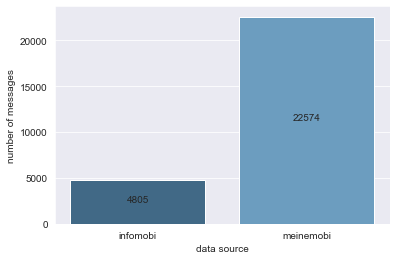
\includegraphics[scale=0.5]{plot-comparison-size}
    \caption{Size comparison of both data sources}
    \label{fig:plot-comparison-size}
\end{figure}

Figure \ref{fig:plot-comparison-size} shows, that the size of \emph{meinemobi} is more than four times larger than the size
of \emph{infomobi}. Before the pre-processing step there is a total number of 27 379 messages. This is a solid base if we
keep in mind, that a large part of the data may be removed at data cleansing. Afterwards, the remaining data needs to be
labelled manually to build a model by supervised learning techniques.

\subsection{Comparison}

There are large differences between these two data sets. The distribution of message types hugely varies between them.
As you can see in figure \ref{fig:plot-comparison-types}, about 80 percent of all messages are of type \emph{HTML}.
This is consistent among the two different data sources. More interesting is the fact, that \emph{infomobi} contains
more \emph{RTF} messages than \emph{Plain Text}, but very few of them are found in \emph{meinemobi}. This is due to
the large number of spam inside \emph{infomobi} which is often formatted as \emph{RTF}. One possible reason for the spam could be,
that the generic email address of \emph{infomobi} is the victim of email harvesting\footnote{The discipline of obtaining email
addresses through various methods like patterns}.

In addition to junk mails, \emph{infomobi} contains a lot more messages in foreign languages than \emph{meinemobi}. These messages
must be removed, so the NLP model will only learn from German. A possible reason might be, that \emph{\textbf{info}@mobiliar.ch}
is more international than the language specific \emph{meinemobi} address.

\begin{figure}[!ht]
    \centering
    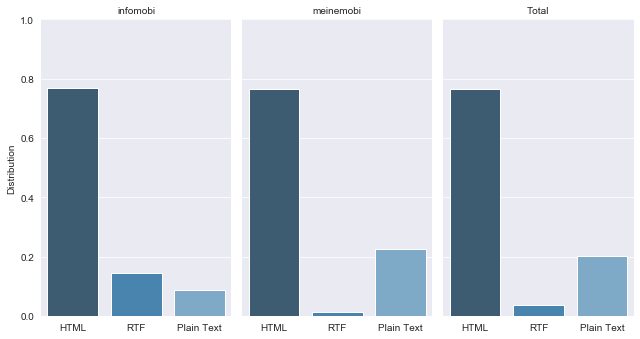
\includegraphics[scale=0.4]{plot-comparison-types}
    \caption{Distribution of the three message types}
    \label{fig:plot-comparison-types}
\end{figure}

Another important key figure is the typical length of a message. This key number can be measured in the total of words or characters.
Figure \ref{fig:plot-comparison-words} shows that the statistical mean of words has to lie somewhere between 186 and 244 words per
message. Due to the size gap between \emph{infomobi} and \emph{meinemobi} the average number of words is therefore about 196.

Figure \ref{fig:plot-comparison-characters} makes it clear that there must be some kind of relation between the number of words
and characters because the two plots looks nearly identical. The division of the number of characters by the amount of words provides
an idea about the typical word in this specific context. Therefore the average word has a length of $8.45$ characters which is much 
higher than the average word in the \emph{\Gls{Duden}} corpus with its length of $6.09$ characters \cite{duden}.

\begin{figure}[!ht]
    \begin{subfigure}{0.5\textwidth}
        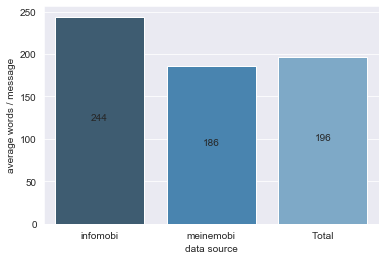
\includegraphics[scale=0.4]{plot-comparison-words} 
        \caption{Comparison of words}
        \label{fig:plot-comparison-words}
    \end{subfigure}
    \begin{subfigure}{0.5\textwidth}
        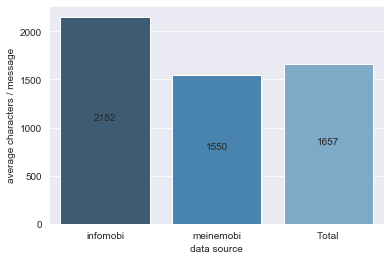
\includegraphics[scale=0.4]{plot-comparison-characters}
        \caption{Comparison of characters}
        \label{fig:plot-comparison-characters}
    \end{subfigure}
    \caption{Comparison of different indicators}
\end{figure}

\subsection{Typical Contents}

Most messages can be divided into different groups. Such groups come very handy at the pre-processing stage when patterns should be
found to locate and remove junk from the remaining information. Therefore the mobi24 data can be splitted into several groups which
are best described with sample messages.

\subsubsection{Spam and Junk}

Junk mails are much harder to detect today than they used to be in the past. Nowadays they are well written and mostly grammatically
correct. Basically you could even use spam to train your model for certain use cases. But in that case spam should consistently be
removed from the data set because it lacks of the insurance context which the model should get familiar with. The presence of links,
the message length and the used language are often good indicators for detecting spam, especially when multiple indicators occur together.

\begin{quote}
    "Ein Ding der Unmöglichkeit! https://zixiseren1983.blogspot.in Auf Wiedersehen Elisabeth Speck"
\end{quote}

\begin{quote}
    "Hallo Ich bin Tony aus Indien. Wir sind ein Team von über 100 IT-Fachleuten mit Fachkenntnissen in folgenden Bereichen: Website-Design, Web-Entwicklung, PHP-Entwicklung, WordPress..."
\end{quote}

\begin{quote}
    "Mit der richtigen Haarpflege zur Traummähne :-) Die besten Pflegeprodukte für jeden Haartyp Endlich schöne Haare! Es ist Zeit, neue Haarprodukte zu entdecken..."
\end{quote}

\subsubsection{Auto-Generated Messages}

Some messages may not origin from real people but from machines instead. These group of messages is called \emph{automatically generated}
and represents the largest group of messages an usual human receives per day. In the data source there are newsletters, notifications
like payment success or delivery messages and failure reports present.

\begin{quote}
    "Fehler bei der Nachrichtenzustellung an folgende Empfänger oder Gruppen: generated1414@mobi.ch Die eingegebene E-Mail-Adresse konnte nicht gefunden werden..."
\end{quote}

\subsubsection{Customer Messages}

For the future model the messages which are actually written by humans and target Swiss Mobiliar's businesses are the only important.
There's a wide range of message types like sponsoring requests, claim notifications, and technical questions. All these messages
share the same context.

Email messages are not as formal as letters and sometimes contain spelling errors. The texts are covered with typical Swiss expressions.
There are even Swiss Mobiliar specific words like the name of products, magazines or applications. It's important to train the future
model on this data to let it become aware of this typical kind of language.

\begin{quote}
    "Geschätzte Mobiliar ich habe mein Passwort verlegt. mit flotten Grüssen N. Augustus"
\end{quote}

\begin{quote}
    "Guten Tag Im Anhang sende ich Ihnen die Offerte zum Schadenfall 8002.2533.9/XX zu. Wir bitten Sie die Offerte zu prüfen. Freundliche Grüsse Tiberius Claudius"
\end{quote}

\begin{quote}
    "Liebe Mobiliar Ich möchte das Mobirama abbestellen. Freundliche Grüsse Julius Bundesgasse 35 3011 Bern"
\end{quote}

\section{Organisation}

This bachelor thesis is written during my last semester at the Bern University of Applied Sciences while I'm working full-time
at the Swiss Mobiliar in the Department of \emph{Cognitive Computing \& Disruptive Analytics}. The department is mainly responsible
for the development of cognitive applications to support existing business processes. They're also trying to establish a
company-wide acceptance through a better understanding of artificial intelligence at Swiss Mobiliar.

\subsection{Coordination}

Swiss Mobiliar is working with the \emph{Atlassian} tool stack. \emph{Jira} is used for keeping track of all unfinished tasks and
dealing with bug requests. The Kanban boards model the current project state by visualising the progress of each story or task.

I'm a member of the agile Scrum team \emph{Aare}\footnote{The beautiful river called Aare floats through the city of Berne}. Because of
Scrum, my colleagues are getting informed about my progress every morning at the daily scrum. At the end of each sprint\footnote{At
Swiss Mobiliar a sprint has a total duration of 3 weeks}, there is a Scrum activity called \emph{Sprint Review} where I present the
latest features to the team.

\begin{figure}[!ht]
\centering
\frame{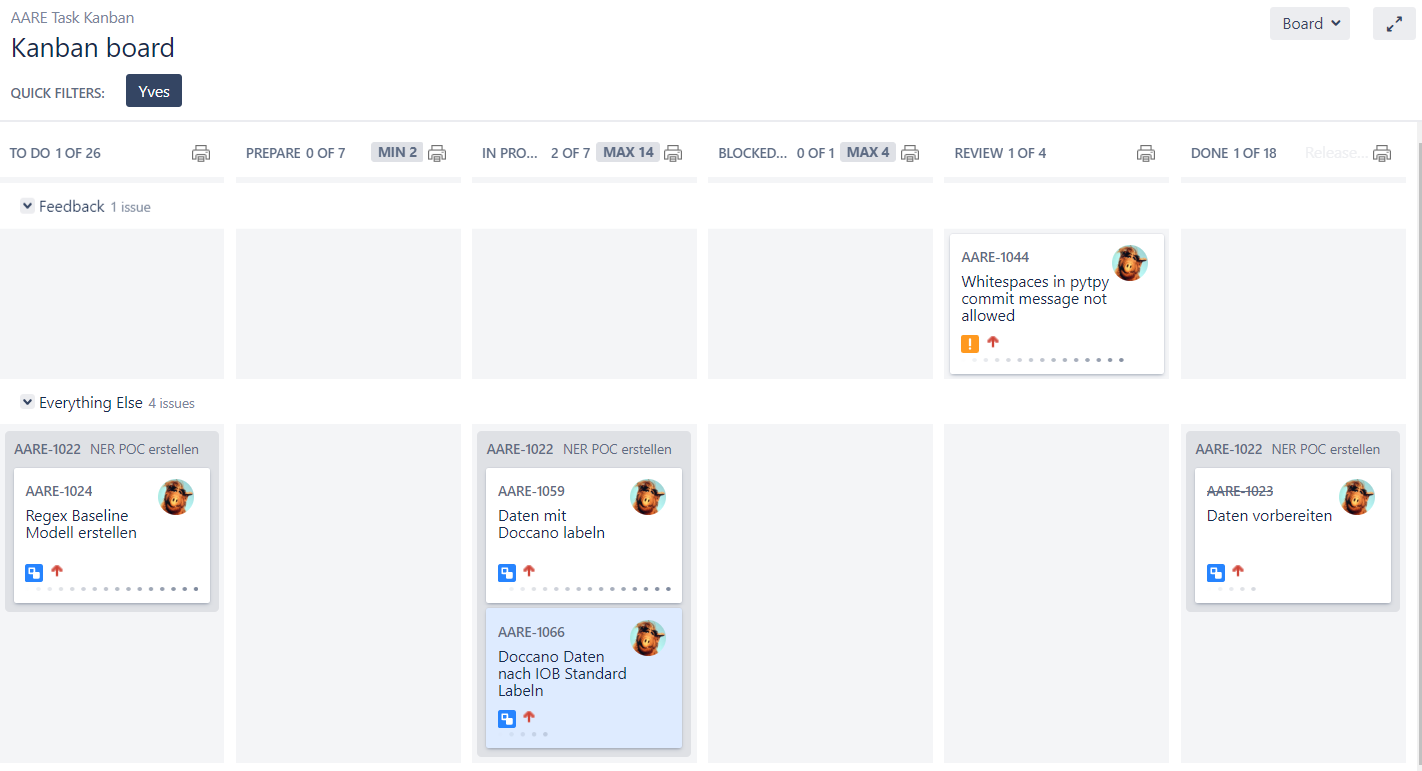
\includegraphics[width=\textwidth]{kanban}}
\caption{View of the Kanban board at an early project stage}
\label{fig:kanban}
\end{figure}

My supervising professor and I organise an informal meeting about every two weeks to discuss the project progress and to plan the
next steps. At this meetup I've got the time to ask questions concerning my current tasks. Due to the short time span between these
meetings, the project itself becomes very agile. I am able to change my primary focus to a different task within weeks.

\subsection{Development Environment}

All source code is generally written in Python. Small code snippets, mostly for exploring and mapping data into another structure,
are created with \emph{jupyter notebooks}. The models and larger pre-processing steps need to be robust and comprehensible, so
unit tests must be created. This code is under version control and will be pushed frequently to the internal Git repository of
Swiss Mobiliar. Teamcity is used as a build server, which controls and deploys the code as a python library. For getting real-world
conditions, the model code is being run inside a docker container\footnote{Tool to run applications inside a container independent
of the underlying operating system}.
